% UQ QOL/EQUS Poster format
% Forked from: https://www.overleaf.com/project/618cc965bcbc81513871601f
% Credit: Ali Furkan Kalay
% See: https://github.com/alfurka/gemini-uq
% Forked from
% https://rev.cs.uchicago.edu/k4rtik/gemini-uccs
% which is forked from
% https://github.com/anishathalye/gemini


\documentclass[final]{beamer}

% ====================
% Packages
% ====================
\usepackage[T1]{fontenc}
\usepackage{lmodern}
\usepackage[orientation=portrait,size=a0,scale=1.0]{beamerposter} % Current dimensions A0, put in your poster dimensions
\usetheme{gemini}
\usecolortheme{uchicago}
\usepackage{graphicx}
\usepackage{caption}
\usepackage{booktabs}
\usepackage{tikz}
\usepackage{pgfplots}
\pgfplotsset{compat=1.17}
\newcommand{\blu}{\color{blue}}
\usepackage{DejaVuSans}
%%%%%%%%%%%%%%%%%%%%%%%%%%%%%%%%%%%%%%%%%%%%%%%%%%%%%%%%%%%%%%%%%%%%%%%%%%%%%%
% Column environment setup
%%%%%%%%%%%%%%%%%%%%%%%%%%%%%%%%%%%%%%%%%%%%%%%%%%%%%%%%%%%%%%%%%%%%%%%%%%%%%%
% If you have N columns, choose \sepwidth and \colwidth such that
% (N+1)*\sepwidth + N*\colwidth = \paperwidth
% Follow structure to create difference column environments. 
\newlength{\sepwidthA} % Seperation distance between comulumns type A
\newlength{\colwidthA} % collumn width type A
\setlength{\sepwidthA}{0.25\paperwidth}
\setlength{\colwidthA}{0.5\paperwidth}

\newcommand{\separatorcolumnA}{\begin{column}{\sepwidthA}\end{column}}

% Second column environment. 
\newlength{\sepwidthB}
\newlength{\colwidthB}
\setlength{\sepwidthB}{0.0666\paperwidth}
\setlength{\colwidthB}{0.4\paperwidth}

\newcommand{\separatorcolumnB}{\begin{column}{\sepwidthB}\end{column}}

% You can also use these column commands to create columns inside columns and for creating new column formatting. 
% You can also have non even columns by creating more column environments or specifying the width when beginning a column environment. 
%%%%%%%%%%%%%%%%%%%%%%%%%%%%%%%%%%%%%%%%%%%%%%%%%%%%%%%%%%%%%%%%%%%%%%%%%%%%%%
% Title
%%%%%%%%%%%%%%%%%%%%%%%%%%%%%%%%%%%%%%%%%%%%%%%%%%%%%%%%%%%%%%%%%%%%%%%%%%%%%%

\title{\VeryHuge{Packet Status Prediction Model \\
Using Packet Sniffer Data}}
\author{Daniel Heráclito Pérez Díaz \and Mariana Ávalos Arce}
\institute[shortinst]{Universidad Panamericana, Guadalajara, México}

%%%%%%%%%%%%%%%%%%%%%%%%%%%%%%%%%%%%%%%%%%%%%%%%%%%%%%%%%%%%%%%%%%%%%%%%%%%%%%
% Poster footer
%%%%%%%%%%%%%%%%%%%%%%%%%%%%%%%%%%%%%%%%%%%%%%%%%%%%%%%%%%%%%%%%%%%%%%%%%%%%%%

\footercontent{
\href{mailto:0190575@up.edu.mx}{0190575@up.edu.mx}
\href{mailto:0197495@up.edu.mx}{0197495@up.edu.mx} % this is a clickable link
  \hfill
  Faculty of Engineering, Data Science \hfill
  {Poster Number: \#1} }
% (can be left out to remove footer)  

\begin{document}
%%%%%%%%%%%%%%%%%%%%%%%%%%%%%%%%%%%%%%%%%%%%%%%%%%%%%%%%%%%%%%%%%%%%%%%%%%%%%%
% Logo placements (optional)
%%%%%%%%%%%%%%%%%%%%%%%%%%%%%%%%%%%%%%%%%%%%%%%%%%%%%%%%%%%%%%%%%%%%%%%%%%%%%%
\addtobeamertemplate{headline}{}
{
    %\begin{tikzpicture}[remember picture,overlay] % Solid header bar
    \begin{tikzpicture}[remember picture,overlay,line width=\arrayrulewidth] % gradient header bar
      % UQ Reverse Logo 
      \node [anchor=north west, inner sep=3cm] at ([xshift=0cm,yshift=1.0cm]current page.north west)
      {\includegraphics[height=8cm]{logos/upwhite02.png}}; 
      % Logo 1, replace with custom logo
      \node [anchor=north east, inner sep=3cm] at ([xshift=0.0cm,yshift=2.0cm]current page.north east)
      {\includegraphics[height=8.0cm]{logos/tree.png}}; 
      % Extra logo 2
      %\node [anchor=north east, inner sep=3cm] at ([xshift=1.0cm,yshift=-10.0cm]current page.north east)
      %{\includegraphics[height=6.0cm]{logos/UQlockup-Purple-cmyk.eps}};
      %  Extra logo 3, or a QR Code
      \node [anchor=north west, inner sep=3cm] at ([xshift=-1.0cm,yshift=-13.0cm]current page.north west)
      {\includegraphics[height=7.0cm]{logos/qr-code.png}}; 
    \end{tikzpicture}
}

% ====================
% Body
% ====================

\begin{frame}[t]
%%%%%%%%%%%%%%%%%%%%%%%%%%%%%%%%%%%%%%%%%%%
%Section 1
%%%%%%%%%%%%%%%%%%%%%%%%%%%%%%%%%%%%%%%%%%%
\begin{columns}[t]
    \separatorcolumnA
    \begin{column}{\colwidthA}

        \begin{block}{Network Topology Proposal}
            \begin{figure}[!Ht]
            \centering
                \includegraphics[width=0.8\linewidth]{Figures/network.png}
                \caption{Network implementing a star topology.}
                \label{fig:top}
            \end{figure}
        \end{block}
    
    \end{column}

    \separatorcolumnA
\end{columns}

%%%%%%%%%%%%%%%%%%%%%%%%%%%%%%%%%%%%%%%%%%%
%Section 2 
%%%%%%%%%%%%%%%%%%%%%%%%%%%%%%%%%%%%%%%%%%%
\begin{columns}
%%%%%%%%%%%%%%%%%%%%%%%%%%%%%%%%%%%%%%%%%%%
%Section 2 column 1
%%%%%%%%%%%%%%%%%%%%%%%%%%%%%%%%%%%%%%%%%%%
\separatorcolumnB

    \begin{column}[T]{\colwidthB}

        \begin{block}{Methodology For Finding Tendency in Data}

        \begin{figure}[!Ht]
            \centering
                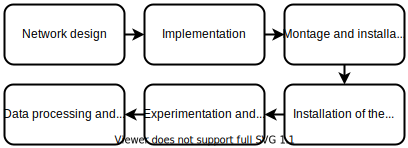
\includegraphics[width=\linewidth]{Figures/method.png}
                \caption{Diagram of the methodology.}
                \label{fig:pipe}
        \end{figure}
    \end{block}
    
    \begin{block}{Hardware}
        The equipment or hardware that will constitute the network to be analyzed are Texas Instruments' Evaluation Boards:

        \begin{figure}[!Ht]
            \centering
                \includegraphics[width=\linewidth]{Figures/hardware.png}
                \caption{Texas Instruments hardware to be used.}
                \label{fig:hw}
        \end{figure}
    \end{block}

    \begin{alertblock}{The Network}
        The protocols implemented by the network are based on IEEE 802.15.4.
    \end{alertblock}
        
\end{column}
\separatorcolumnB
%%%%%%%%%%%%%%%%%%%%%%%%%%%%%%%%%%%%%%%%%%%
%Section 2 column 2
%%%%%%%%%%%%%%%%%%%%%%%%%%%%%%%%%%%%%%%%%%%
\begin{column}[T]{\colwidthB}

    \begin{block}{Applications}
    An IoT (internet of Things) development example are Smart Cities, where these are defined as the quality of living improvement through the use of hardware, software, networks and data. The question that the prediction model would answer on a wider scale would be if, on a Smart City, whose network is presenting packet loss, the real need is \textit{more routers} or simply a \textit{rearrangement of the network's nodes}, coming from the type of interference it presents.

        \begin{figure}[!Ht]
            \centering
                \includegraphics[width=0.7\linewidth]{Figures/smart-city-app.png}
                \caption{Smart City node rearrangement.}
                \label{fig:app}
        \end{figure}
    \end{block}

  

    

%%%%%%%%%%%%%%%%%%%%%%%%%%%%%%%%%%%%%%%%%%%%%%%%%%%%%%%%%%%%%%%%%%%%%%%%%%%%%%
% References
%%%%%%%%%%%%%%%%%%%%%%%%%%%%%%%%%%%%%%%%%%%%%%%%%%%%%%%%%%%%%%%%%%%%%%%%%%%%%%
\begin{block}{References}

\nocite{*}
\bibliography{poster}% Produces the bibliography via BibTeX.
\bibliographystyle{plain}
\end{block} 

\end{column}
\separatorcolumnB
\end{columns}
\end{frame}
\end{document}
